\documentclass[border=5pt]{standalone}
\usepackage[utf8]{inputenc}
\usepackage{amssymb}
\usepackage{amsmath}
\usepackage{tikz}
\usetikzlibrary{arrows.meta}

\begin{document}
\nopagecolor
\begin{tabular}{c c}
    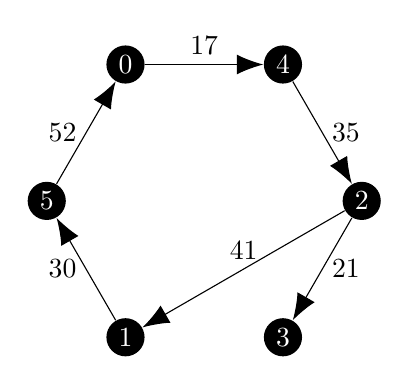
\begin{tikzpicture}
        \node[circle, inner sep=2pt, fill] (0) at (-1, 1.732) {\color{white} 0};
        \node[circle, inner sep=2pt, fill] (4) at (1, 1.732) {\color{white} 4};
        \node[circle, inner sep=2pt, fill] (2) at (2, 0) {\color{white} 2};
        \node[circle, inner sep=2pt, fill] (3) at (1, -1.732) {\color{white} 3};
        \node[circle, inner sep=2pt, fill] (1) at (-1, -1.732) {\color{white} 1};
        \node[circle, inner sep=2pt, fill] (5) at (-2, 0) {\color{white} 5};
        
        \draw[-{Latex[scale=2]}] (1) edge[left] node{30} (5);
        \draw[-{Latex[scale=2]}] (2) edge[above] node{41} (1);
        \draw[-{Latex[scale=2]}] (2) edge[right] node{21} (3);
        \draw[-{Latex[scale=2]}] (4) edge[right] node{35} (2);
        \draw[-{Latex[scale=2]}] (5) edge[left] node{52} (0);
        \draw[-{Latex[scale=2]}] (0) edge[above] node{17} (4);
    \end{tikzpicture}
    &
    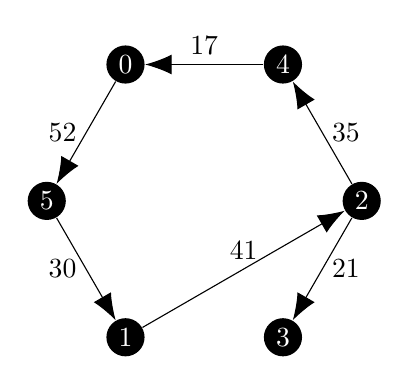
\begin{tikzpicture}
        \node[circle, inner sep=2pt, fill] (0) at (-1, 1.732) {\color{white} 0};
        \node[circle, inner sep=2pt, fill] (4) at (1, 1.732) {\color{white} 4};
        \node[circle, inner sep=2pt, fill] (2) at (2, 0) {\color{white} 2};
        \node[circle, inner sep=2pt, fill] (3) at (1, -1.732) {\color{white} 3};
        \node[circle, inner sep=2pt, fill] (1) at (-1, -1.732) {\color{white} 1};
        \node[circle, inner sep=2pt, fill] (5) at (-2, 0) {\color{white} 5};
        
        \draw[{Latex[scale=2]}-] (1) edge[left] node{30} (5);
        \draw[{Latex[scale=2]}-] (2) edge[above] node{41} (1);
        \draw[-{Latex[scale=2]}] (2) edge[right] node{21} (3);
        \draw[{Latex[scale=2]}-] (4) edge[right] node{35} (2);
        \draw[{Latex[scale=2]}-] (5) edge[left] node{52} (0);
        \draw[{Latex[scale=2]}-] (0) edge[above] node{17} (4);
    \end{tikzpicture}
    \\
    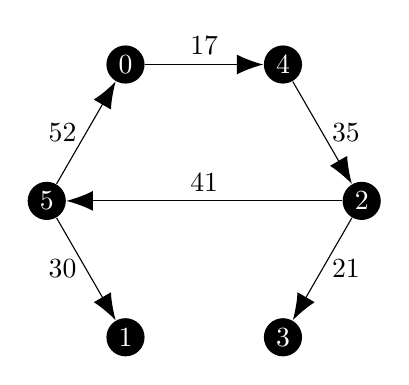
\begin{tikzpicture}
        \node[circle, inner sep=2pt, fill] (0) at (-1, 1.732) {\color{white} 0};
        \node[circle, inner sep=2pt, fill] (4) at (1, 1.732) {\color{white} 4};
        \node[circle, inner sep=2pt, fill] (2) at (2, 0) {\color{white} 2};
        \node[circle, inner sep=2pt, fill] (3) at (1, -1.732) {\color{white} 3};
        \node[circle, inner sep=2pt, fill] (1) at (-1, -1.732) {\color{white} 1};
        \node[circle, inner sep=2pt, fill] (5) at (-2, 0) {\color{white} 5};
        
        \draw[-{Latex[scale=2]}] (2) edge[right] node{21} (3);
        \draw[{Latex[scale=2]}-] (2) edge[right] node{35} (4);
        \draw[{Latex[scale=2]}-] (4) edge[above] node{17} (0);
        \draw[-{Latex[scale=2]}] (5) edge[left] node{30} (1);
        \draw[{Latex[scale=2]}-] (5) edge[above] node{41} (2);
        \draw[{Latex[scale=2]}-] (0) edge[left] node{52} (5);
    \end{tikzpicture}
    &
    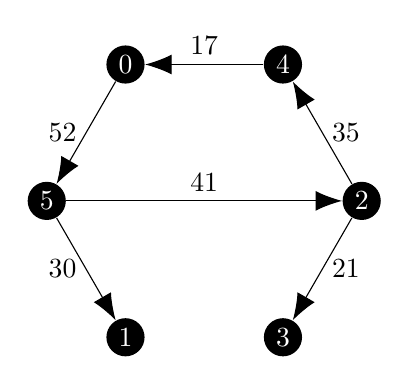
\begin{tikzpicture}
        \node[circle, inner sep=2pt, fill] (0) at (-1, 1.732) {\color{white} 0};
        \node[circle, inner sep=2pt, fill] (4) at (1, 1.732) {\color{white} 4};
        \node[circle, inner sep=2pt, fill] (2) at (2, 0) {\color{white} 2};
        \node[circle, inner sep=2pt, fill] (3) at (1, -1.732) {\color{white} 3};
        \node[circle, inner sep=2pt, fill] (1) at (-1, -1.732) {\color{white} 1};
        \node[circle, inner sep=2pt, fill] (5) at (-2, 0) {\color{white} 5};
        
        \draw[-{Latex[scale=2]}] (2) edge[right] node{21} (3);
        \draw[-{Latex[scale=2]}] (2) edge[right] node{35} (4);
        \draw[-{Latex[scale=2]}] (4) edge[above] node{17} (0);
        \draw[-{Latex[scale=2]}] (5) edge[left] node{30} (1);
        \draw[-{Latex[scale=2]}] (5) edge[above] node{41} (2);
        \draw[-{Latex[scale=2]}] (0) edge[left] node{52} (5);
    \end{tikzpicture}
    \\
    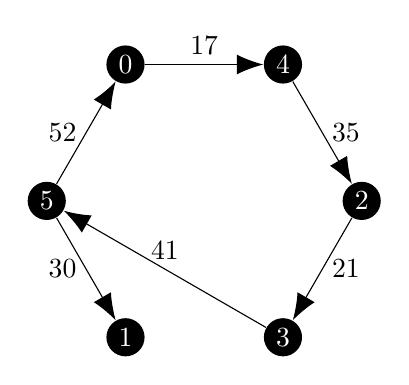
\begin{tikzpicture}
        \node[circle, inner sep=2pt, fill] (0) at (-1, 1.732) {\color{white} 0};
        \node[circle, inner sep=2pt, fill] (4) at (1, 1.732) {\color{white} 4};
        \node[circle, inner sep=2pt, fill] (2) at (2, 0) {\color{white} 2};
        \node[circle, inner sep=2pt, fill] (3) at (1, -1.732) {\color{white} 3};
        \node[circle, inner sep=2pt, fill] (1) at (-1, -1.732) {\color{white} 1};
        \node[circle, inner sep=2pt, fill] (5) at (-2, 0) {\color{white} 5};
        
        \draw[-{Latex[scale=2]}] (2) edge[right] node{21} (3);
        \draw[-{Latex[scale=2]}] (3) edge[above] node{41} (5);
        \draw[-{Latex[scale=2]}] (4) edge[right] node{35} (2);
        \draw[-{Latex[scale=2]}] (5) edge[left] node{30} (1);
        \draw[-{Latex[scale=2]}] (5) edge[left] node{52} (0);
        \draw[-{Latex[scale=2]}] (0) edge[above] node{17} (4);
    \end{tikzpicture}
    &
    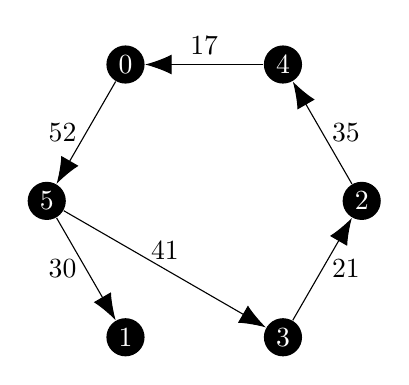
\begin{tikzpicture}
        \node[circle, inner sep=2pt, fill] (0) at (-1, 1.732) {\color{white} 0};
        \node[circle, inner sep=2pt, fill] (4) at (1, 1.732) {\color{white} 4};
        \node[circle, inner sep=2pt, fill] (2) at (2, 0) {\color{white} 2};
        \node[circle, inner sep=2pt, fill] (3) at (1, -1.732) {\color{white} 3};
        \node[circle, inner sep=2pt, fill] (1) at (-1, -1.732) {\color{white} 1};
        \node[circle, inner sep=2pt, fill] (5) at (-2, 0) {\color{white} 5};
        
        \draw[{Latex[scale=2]}-] (2) edge[right] node{21} (3);
        \draw[{Latex[scale=2]}-] (3) edge[above] node{41} (5);
        \draw[{Latex[scale=2]}-] (4) edge[right] node{35} (2);
        \draw[-{Latex[scale=2]}] (5) edge[left] node{30} (1);
        \draw[{Latex[scale=2]}-] (5) edge[left] node{52} (0);
        \draw[{Latex[scale=2]}-] (0) edge[above] node{17} (4);
    \end{tikzpicture}
    \\
\end{tabular}
\end{document}